\clearpage
\chapter{轨道角动量算符}	\label{A03}

在直角坐标系中,以$\boldsymbol{e}_{1},\boldsymbol{e}_{2},\boldsymbol{e}_{3}$表示$x,y,z$轴方向单位矢量.粒子的位置矢量和梯度算符可以表示成
\begin{empheq}{align}
	&\boldsymbol{r}=x\boldsymbol{e}_{1}+y\boldsymbol{e}_{2}+z\boldsymbol{e}_{3}		\label{eqA3.1}\\
	\nabla&=\boldsymbol{e}_{1}\frac{\partial}{\partial x}+\boldsymbol{e}_{2}\frac{\partial}{\partial y}+\boldsymbol{e}_{3}\frac{\partial}{\partial z}		\label{eqA3.2}
\end{empheq}\eqlong
\begin{wrapfigure}[15]{r}{0.3\textwidth}
	\centering
	\small
	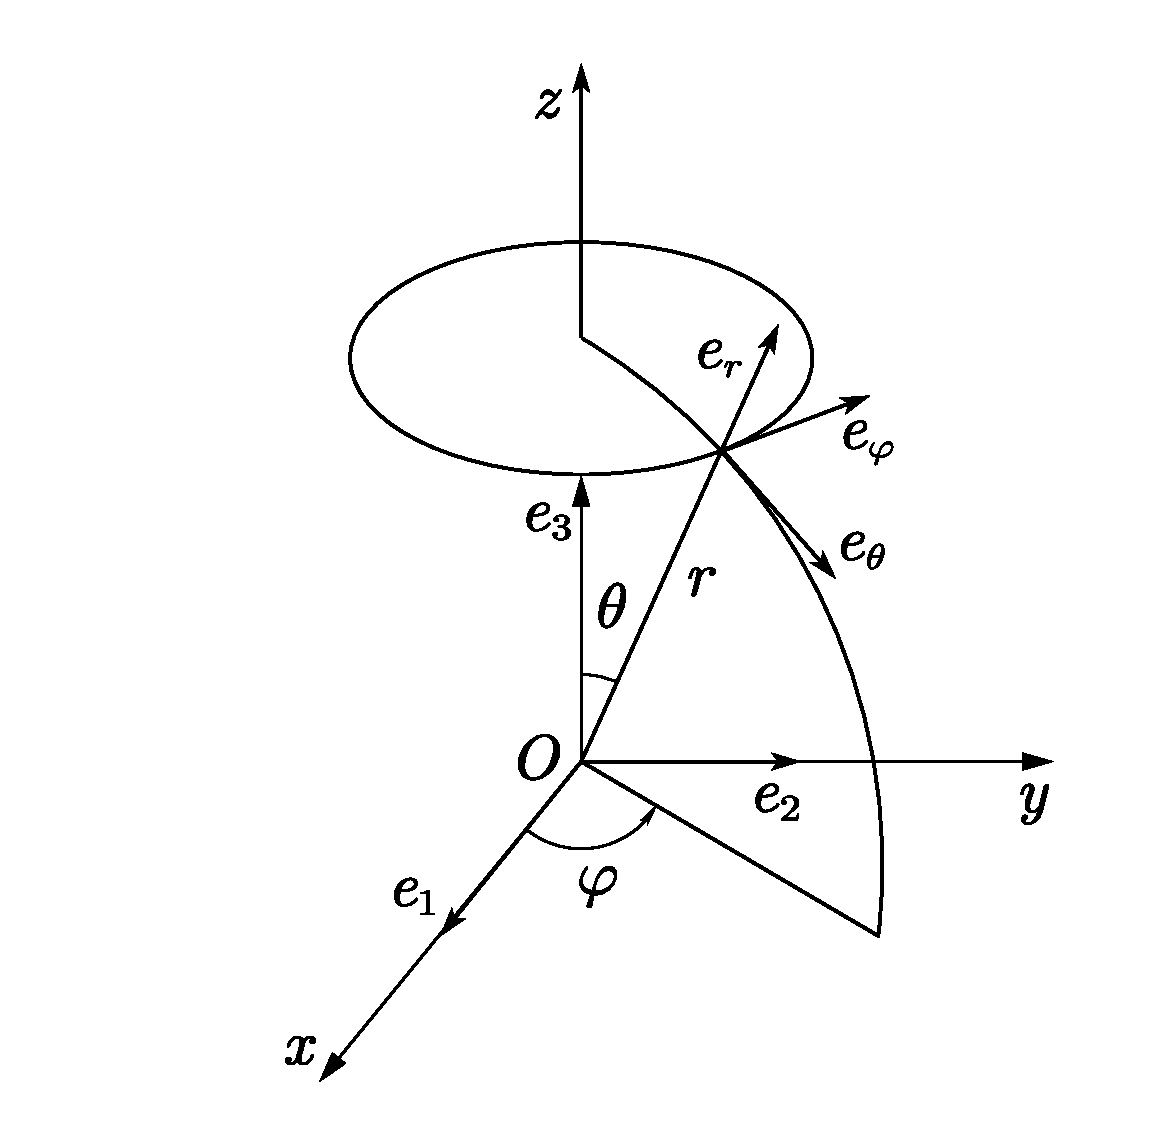
\includegraphics[width=3.5cm,clip]{QM file/figure/A-3}
	\caption*{附录图3}\label{fig.A-3}
\end{wrapfigure}

\noindent 轨道角动量算符为
\begin{empheq}{equation}\label{eqA3.3}
	\boldsymbol{L}=\boldsymbol{r}\times\boldsymbol{p}=-i\hbar\boldsymbol{r}\times\nabla
\end{empheq}\eqindent{1}

在球坐标系中,以$\boldsymbol{e}_{r},\boldsymbol{e}_{\theta},\boldsymbol{e}_{\varphi}$分别表示沿径向,经线切线方向,纬线切线方向单位矢量(附录图3),三者有关系
\begin{equation}\label{eqA3.4}
	\boldsymbol{e}_{r}\times\boldsymbol{e}_{\theta}=\boldsymbol{e}_{\varphi},\quad \boldsymbol{e}_{\theta}\times\boldsymbol{e}_{\varphi}=\boldsymbol{e}_{r},\quad \boldsymbol{e}_{\varphi}\times\boldsymbol{e}_{r}=\boldsymbol{e}_{\theta}
\end{equation}\eqlllong
梯度$\nabla$的球坐标表示为
\begin{equation}\label{eqA3.5}
	\nabla=\boldsymbol{e}_{r}\frac{\partial}{\partial r}+\boldsymbol{e}_{\theta}\frac{1}{r}\frac{\partial}{\partial\theta}+\boldsymbol{e}_{\varphi}\frac{1}{r\sin\theta}\frac{\partial}{\partial\varphi}
\end{equation}\eqnormal
因此,轨道角动量算符可以表示成
\begin{empheq}{align}\label{eqA3.6}
	\boldsymbol{L}&=-i\hbar r\boldsymbol{e}_{r}\times\nabla	\nonumber\\
	&=-i\hbar\left(\boldsymbol{e}_{\varphi}\frac{\partial}{\partial\theta}-\boldsymbol{e}_{\theta}\frac{1}{\sin\theta}\frac{\partial}{\partial\varphi}\right)
\end{empheq}
分别取上式与$\boldsymbol{e}_{1},\boldsymbol{e}_{2},\boldsymbol{e}_{3}$的内积,并注意到
\begin{empheq}{align}\label{eqA3.7}
	\boldsymbol{e}_{1}\cdot\boldsymbol{e}_{\theta}=&\cos\theta\cos\varphi,\quad \boldsymbol{e}_{1}\cdot\boldsymbol{e}_{\varphi}=-\sin\varphi \nonumber\\
	\boldsymbol{e}_{2}\cdot\boldsymbol{e}_{\theta}=&\cos\theta\sin\varphi,\quad \boldsymbol{e}_{2}\cdot\boldsymbol{e}_{\varphi}=\cos\varphi	\nonumber\\
	(&\boldsymbol{e}_{1}\pm i\boldsymbol{e}_{2})\cdot\boldsymbol{e}_{\theta}=\cos\theta\boldsymbol{e}^{\pm i\varphi}	\nonumber\\
	&(\boldsymbol{e}_{1}\pm i\boldsymbol{e}_{2})\cdot\boldsymbol{e}_{\varphi}=\pm i\boldsymbol{e}^{\pm i\varphi}	\nonumber\\		
	\boldsymbol{e}_{3}\cdot\boldsymbol{e}_{\theta}=&-\sin\theta,\quad \boldsymbol{e}_{3}\cdot\boldsymbol{e}_{\varphi}=0
\end{empheq}\eqindent{8}
即得
\begin{empheq}{align}
	L_{x}&=i\hbar\left(\sin\varphi\frac{\partial}{\partial\theta}+\cot\theta\cos\varphi\frac{\partial}{\partial\varphi}\right)		\nonumber\\
	L_{y}&=i\hbar\left(-\cos\varphi\frac{\partial}{\partial\theta}+\cot\theta\sin\varphi\frac{\partial}{\partial\varphi}\right)	\label{eqA3.8}\\
	L_{x}&\pm iL_{y}=\hbar e^{\pm i\varphi}\left(\pm\frac{\partial}{\partial\theta}+i\cot\theta\frac{\partial}{\partial\varphi}\right)		\label{eqA3.9}\\
	L_{z}&=-i\hbar\frac{\partial}{\partial\varphi}		\label{eqA3.10}
\end{empheq}
另外,$\boldsymbol{L}^{2}$可以表示成
\begin{empheq}{align}\label{eqA3.11}
	\boldsymbol{L}^{2}&=L_{x}^{2}+L_{y}^{2}+L_{z}^{2}	\nonumber\\
	&(L_{x}-iL_{y})(L_{z}+iL_{y})+\hbar L_{z}+L_{z}^{2}
\end{empheq}
(利用$L_{x}L_{y}-L_{y}L_{x}=i\hbar L_{z}$)将\eqref{eqA3.9}、\eqref{eqA3.10}式代入上式,经过化简,即得
\begin{empheq}{align}\label{eqA3.12}
	\boldsymbol{L}^{2}&=-\hbar^{2}\left(\frac{\partial^{2}}{\partial\theta^{2}}+\cot\theta\frac{\partial}{\partial\theta}+\frac{1}{\sin^{2}\theta}\frac{\partial^{2}}{\partial\varphi^{2}}\right)	\\
	&=-\hbar^{2}\left(\frac{1}{\sin\theta}\frac{\partial}{\partial\theta}\sin\theta\frac{\partial}{\partial\theta}+\frac{1}{\sin^{2}\theta}\frac{\partial^{2}}{\partial\varphi^{2}}\right)
\end{empheq}\eqlong
采用球坐标时,常令$\cos\theta=\xi$,而以$(r,\xi,\varphi)$作为坐标变量,这时\eqref{eqA3.9}式及\eqref{eqA3.12}式变成
\begin{empheq}{align}
	L_{x}\pm iL_{y}=\hbar e^{\pm i\varphi}\left[\mp(1-\xi^{2})^{\frac{1}{2}}\frac{\partial}{\partial\xi}+i\xi(1-\xi^{2})^{-\frac{1}{2}}\frac{\partial}{\partial\varphi}\right]		\label{eqA3.13}\\
	\boldsymbol{L}^{2}=-\hbar^{2}\left[(1-\xi^{2})\frac{\partial^{2}}{\partial\xi^{2}}-2\xi\frac{\partial}{\partial\xi}+(1-\xi^{2})^{-1}\frac{\partial^{2}}{\partial\varphi^{2}}\right]		\label{eqA3.14}
\end{empheq}\eqnormal